%!TEX root = ../main.tex

\section{Local Storage}
In addition to transmitting data to a stationary computer, the data should be stored on the go-kart.
It should be possible to transmit this data through WiFi upon request.
This will ensure, that no data is lost if the go-kart gets out of range of the WiFi.
The storage will be done on the WiFi node as transmitting a potentially large log over the CAN bus could potentially be inefficient.\\

Each Zybo has an SD card which holds the operating system.
These particular SD cards have more than 3 GB of un-partitioned space which can be used for log storage. 
Linux allows for an easy way to handle files, which would ease the task of logging data at fixed intervals, or to read the log back.
At this point, it is not clear how much data will be on the bus, which means that it is not clear whether this is enough.
The assumption is made that data will be stored only for one drive session.
That is, upon starting a new drive, the old log is deleted.
This assumption enables calculating the maximum writing speed possible while not running out of space.\\

From experience, it is known, that the go-kart has battery for half an hour driving sessions.
From this knowledge, the data rate can be calculated as follows:

\begin{equation}
	\frac{3\mathrm{GB}}{30\si{\minute}} = \frac{2.58 \cdot 10^{10} \mathrm{bit}}{1800 \si{\second}} \approx 13.7 \mathrm{Mb/s}
\end{equation}

With a data rate this high, it is unlikely that the go-kart runs out of storage space before it runs out of battery.

\section{Software on Stationary Computer}
The stationary computer needs to receive data through WiFi and decode the received messages using the protocol that is to be developed.
A user should be able to access the data through an API.
This API should act as the front end of the underlying network.
As a proof of concept, a simple UI should be implemented to show how data can be presented to the user.
The software also needs the ability to let the user send a command to the on-vehicle network to start and stop specific nodes.
As with the previous parts of the system, this program should be compatible with Linux.
The described software is outlined in figure \ref{fig:setup_ui}.

\begin{figure}[h]
	\centering
	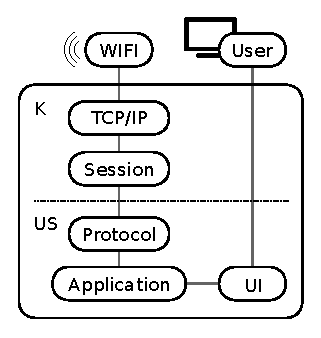
\includegraphics{graphics/stationary_software.eps}
	\caption{Structure of software on stationary computer.}
	\label{fig:setup_ui}
\end{figure}

\subsection{Protocol}
As described in section \ref{sec:canbusanalysis}, a custom protocol will be developed to complement CAN.
Any data received through the WiFi will be encoded using this protocol.
It is the responsibility of this software to decode the software in order to present it to the user in a readable format.
In order to maintain the modularity of the system, the decoding should be done in such a way that future developers can easily add new nodes, and with them, new decoding for data types.

\subsection{Application}
The system is intended to function as a monitoring system of go-kart data.
Presentation of the data is not the focus of the project and as such only a rudimentary UI is developed to show the functionality.
The software should however be designed in such a way that a developer can easily create a custom (G)UI for the system, which fits the needs of that particular project.
In order to create the most seamless interface for this functionality the software should implement an API which acts as a front end for the underlying network.
The API-approach has the added benefit of allowing the user to use the incoming data in any way that may suit their project.
